\section{Textursynthese}

Die \emph{Textursynthese} ist ein alternativer Ansatz für die Erstellung von Texturen, der es erlaubt, auch ohne spezielle Vorkenntnisse, qualitativ hochwertige Ergebnisse zu erzielen.
Der Benutzer muss lediglich ein Beispielmuster und eventuell benötigte Konfigurationsparameter an die Textursynthese übergeben, die aus diesen Daten eine Textur synthetisiert \cite{StateOfTheArt}.
Die resultierende Textur zeichnet sich dadurch aus, dass sie eine beliebige Größe annehmen kann, aber weiterhin sichtbare Ähnlichkeiten zu dem Beispielmuster aufweist ohne identisch zu ihm zu sein.
Die Textursynthese kümmert sich dabei automatisiert und im Idealfall ohne technische Benutzereingaben um die Schwierigkeiten bei der Erstellung von Texturen.
Sie berücksichtigt die visuellen Charakteristiken des Beispielmusters und vermeidet dabei zeitgleich auffällige Wiederholungen oder Unnatürlichkeiten in der synthetisierten Textur.

\subsection{\glqq Markov Random Fields\grqq -Eigenschaft}

Die \emph{\glqq Markov Random Field\grqq} -Eigenschaft ist eine der populärsten Eigenschaften, die vielen Verfahren der Textursynthese zu Grunde liegt \cite{StateOfTheArt}.
Sie motiviert eine Metrik, die Verwendung findet, um die Ähnlichkeit zwischen dem Beispielmuster und der zu synthetisierenden Textur zu beschreiben \cite{TextureOptimization}.
Die \glqq Markov Random Field\grqq -Eigenschaft beschreibt dabei die Synthese als eine Aneinanderreihung von \emph{lokalen} und \emph{stationären} Prozessen \cite{StateOfTheArt}.
Das bedeutet, dass jede Farbe eines Pixels in der Textur ausschließlich über die Pixel in seiner direkten räumlichen Nachbarschaft charakterisiert werden kann (lokal).
Diese Charakterisierung ist dabei unabhängig von der Position des betrachteten Pixels (stationär) \cite{TextureOptimization}.
Die Intuition dieser Eigenschaft lässt sich anhand von einem Beispiel verdeutlichen (vgl. Abbildung \ref{mrf}).
Einem Betrachter liegt ein Bild vor, welches er aber nur durch ein kleines bewegliches Fenster betrachten kann.
Er sieht demnach nie das komplette Bild auf einmal, kann aber durch Bewegungen seines Fensters einzelne Bereiche des Bildes entdecken und erschließen.
Das Bild ist dann stationär, falls es unter verschiedenen Ausschnitten immer ähnlich erscheint (eine geeignete Fenstergröße vorausgesetzt).
Das Bild ist lokal, falls jeder Pixel in der Mitte eines Fensters über die umliegenden Pixel in seinem Fenster bestimmt werden kann \cite{StateOfTheArt}.

\begin{figure}
	\centering
	\begin{subfigure}{0.45\textwidth}
		\centering
		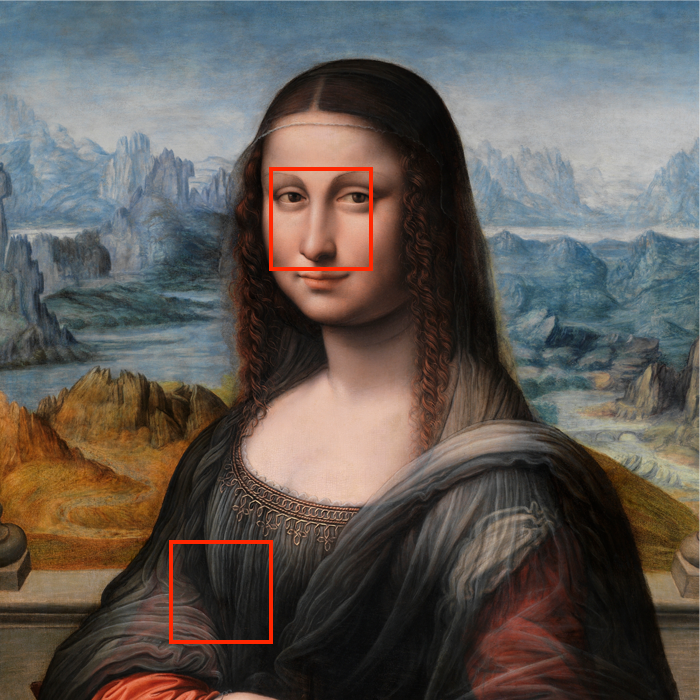
\includegraphics[width=0.7\textwidth]{images/mrf-1}
		\caption*{($a$)}
		
		\begin{subfigure}{0.45\textwidth}
			\centering
			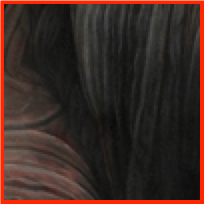
\includegraphics[width=0.5\textwidth]{images/mrf-1-1}
			\caption*{($a_1$)}
		\end{subfigure}
		\hfill
		\begin{subfigure}{0.45\textwidth}
			\centering
			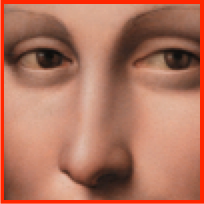
\includegraphics[width=0.5\textwidth]{images/mrf-1-2}
			\caption*{($a_2$)}
		\end{subfigure}
		
	\end{subfigure}
	\hfill
	\begin{subfigure}{0.45\textwidth}
		\centering
		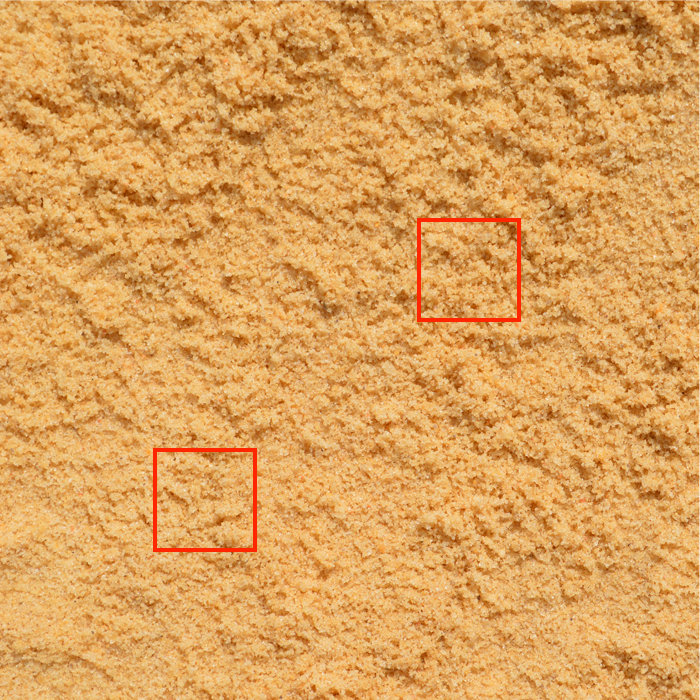
\includegraphics[width=0.7\textwidth]{images/mrf-2}
		\caption*{($b$)}
		
		\begin{subfigure}{0.45\textwidth}
			\centering
			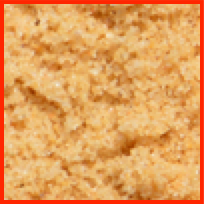
\includegraphics[width=0.5\textwidth]{images/mrf-2-1}
			\caption*{($b_1$)}
		\end{subfigure}
		\hfill
		\begin{subfigure}{0.45\textwidth}
			\centering
			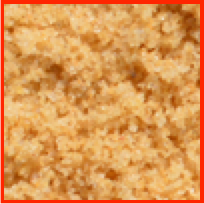
\includegraphics[width=0.5\textwidth]{images/mrf-2-2}
			\caption*{($b_2$)}
		\end{subfigure}
		
	\end{subfigure}
	
	\caption{
		($a$) ist ein generelles Bild während ($b$) eine Textur ist.
		Ein bewegliches Fenster an zwei unterschiedlichen Positionen ist als rotes Quadrat in ($a$) und ($b$) gekennzeichnet.
		Unterschiedliche Aussschnitte einer Textur sind sichtbar ähnlich zueinander sein ($b_1$, $b_2$).
		Dies ist nicht der Fall für ein generelles Bild ($a_1$, $a_2$).
	}
	\label{mrf}
\end{figure}

Basierend auf dieser Eigenschaft kann der Prozess der Textursynthese spezifiziert werden.
Sei ein Beispielmuster gegeben.
Dann lässt sich daraus eine Textur synthetisieren, sodass für jeden synthetisierten Pixel dessen räumliche Nachbarschaft zu mindestens einer Nachbarschaft im Beispielmuster ähnlich ist \cite{StateOfTheArt}.
Die Größe der betrachteten Nachbarschaften ist dabei in der Regel ein benutzerdefinierter Parameter.
Die Nachbarschaftssuche basiert im Allgemeinen auf der kleinsten quadrierten farblichen Abweichung 

\begin{equation}
	\label{nachbarschaftssuche}
	\min d(\textbf{t}_i, \textbf{x}_j) = \lVert \textbf{t}_i - \textbf{x}_j \rVert^2\text{.}
\end{equation}

$\textbf{t}_i$ beziehungsweise $\textbf{x}_j$ beschreiben dabei die Farben einer Nachbarschaft der Größe $N \times N$ als Vektor um den Pixel $i$ in der Textur $T$ respektive um den Pixel $j$ in dem Beispielmuster $X$.
Für jede Nachbarschaft $\textbf{t}_i$ ist dann ihre ähnlichste Nachbarschaft $\textbf{x}_j$ im Beispielmuster gefunden, wenn $d(\textbf{t}_i, \textbf{x}_j)$ minimal ist \cite{TextureOptimization}.

Aufgrund der Ähnlichkeiten zwischen lokalen Nachbarschaften im Beispielmuster und der Textur wird garantiert, dass die synthetisierte Textur Gemeinsamkeiten mit dem Beispielmuster aufweist \cite{StateOfTheArt}.

\subsection{Verfahren}

Der Großteil an veröffentlichten Algorithmen zur Textursynthese basiert auf der \glqq Markov Random Fields\grqq -Eigenschaft \cite{StateOfTheArt}.
Diese Verfahren lassen sich in der Regel einer von zwei Kategorien zuordnen: den \emph{lokal wachsenden Verfahren} und den \emph{global optimierenden Verfahren}.
Lokal wachsende Verfahren synthetisieren die Textur nach und nach über einzelne Pixel oder Regionen \cite{TextureOptimization}.
Global optimierende Verfahren hingegen synthetisieren und optimieren die Textur iterativ als Ganzes auf Basis einer Zielfunktion \cite{SelfTuning}.
Im Folgenden sollen drei Verfahren der beiden Kategorien näher betrachtet werden.

\subsubsection{Pixelbasierte Textursynthese}

Einer der ersten Ansätze der Textursynthese ist die \emph{pixelbasierte Textursynthese} (vgl. \cite{EL99}).
Er fällt in die Kategorie der lokal wachsenden Verfahren.
Sei ein Beispielmuster und eine Nachbarschaftsgröße gegeben, dann funktioniert die grundlegende Idee hinter diesem Algorithmus wie folgt.

\begin{figure}
	\centering
	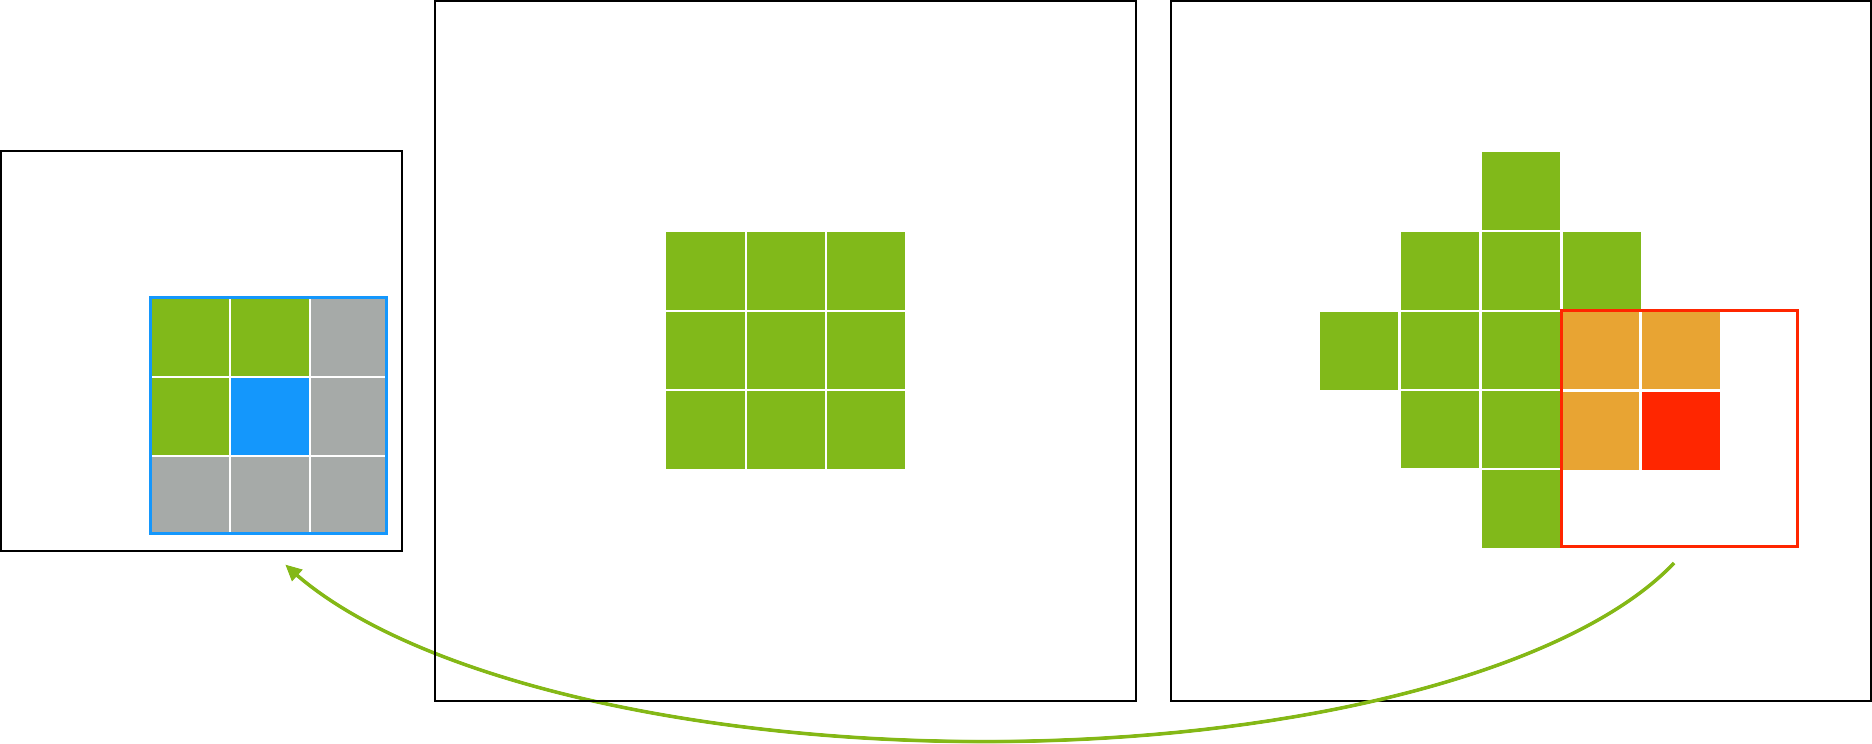
\includegraphics[width=0.85\textwidth]{images/pixelbased}
	\caption{
		Der Algorithmus von \cite{EL99}.
		Aus einem Beispielmuster (links) wird zuerst eine initiale Textur erstellt, indem eine kleine Region aus dem Beispielmuster in diese kopiert wird (Mitte). Der Algorithmus berechnet die Pixel dann sukzessive um die initiale Region auf Basis der Nachbarschaftssuche (rechts).
	}
	\label{pixelbased}
\end{figure}

Die zu synthetisierende Textur wird zuerst initialisiert, indem eine kleine beliebige Region des Beispielmusters in die Mitte der Textur kopiert wird.
Der Algorithmus berechnet dann sukzessive die einzelnen Pixelfarben der Textur kreisförmig um die initiale Region von innen nach außen.
Abbildung \ref{pixelbased} illustriert dieses Verfahren.
Die Farbe eines aktuell betrachteten Pixels $p$ (rot) in der Textur wird dann über eine Nachbarschaftssuche im Beispielmuster ermittelt.
Dazu wird zuerst ein Rahmen mit der Größe der Nachbarschaft um den Pixel $p$ gelegt (hier $3 \times 3$) und alle bereits gesetzten Pixel in diesem Rahmen gefunden (orange).
Auf Basis dieser gesetzten Pixel wird im Beispielmuster die ähnlichste Nachbarschaft auf Grundlage von (\ref{nachbarschaftssuche}) gefunden.
Der Pixel $p$ erhält dann die Farbe des Pixels in der Mitte der ermittelten ähnlichsten Nachbarschaft im Beispielmuster (blau).
Dieser Vorgang wird solange wiederholt, bis alle Pixel der Textur gesetzt sind.

Der Algorithmus \cite{EL99} ist relativ einfach zu verstehen sowie zu implementieren \cite{StateOfTheArt}.
Er ist außerdem benutzerfreundlich, da dieser lediglich einen Konfigurationsparameter, die Nachbarschaftsgröße, an den Algorithmus übergeben muss \cite{EL99}.
Die Wahl der Nachbarschaftsgröße ist jedoch nicht trivial.
Fällt die Wahl der Nachbarschaftsgröße zu klein aus, so kann das Ergebnis zu zufällig wirken.
Ist sie auf der anderen Seite zu groß, können sichtbare Wiederholungen entstehen oder es kommt zu Unnatürlichkeiten, da die Nachbarschaftssuche auf Grund ihrer Größe wohlmöglich keine geeigneten Kandidaten finden kann \cite{StateOfTheArt}.

\subsubsection{Regionsbasierte Textursynthese}

Ein weiterer Vertreter der lokal wachsenden Verfahren und eine Erweiterung bzw. ein Nachfolger der pixelbasierten Textursynthese ist die \emph{regionsbasierte Textursynthese} (vgl. \cite{StateOfTheArt}).
Die regionsbasierte Synthese ist sehr ähnlich zu der pixelbasierten Synthese, aber anstatt einzelne Pixel zu kopieren, werden stattdessen ganze Regionen in die Textur kopiert.
Damit kann die Qualität der Textursynthese verbessert werden, denn es ist sichergestellt, dass Pixel innerhalb einer Region auch zueinander passen.
Der wesentliche Unterschied der beiden Verfahren besteht letztendlich im Kopierungsprozess.
In pixelbasierten Algorithmen ist die Kopie eines Pixels fest und kann nachträglich nicht mehr verändert werden.
Bei den regionsbasierten Verfahren verhält es sich anders, da die Kopie einer Region üblicherweise dazu führt, dass bereits synthetisierte Bereiche der Textur durch die neue Region überdeckt werden.
Der Algorithmus muss folglich eine Entscheidung treffen, wie er mit den im Konflikt stehenden Pixeln umgeht.
Mehrere mögliche Szenarien sind die Folge.
Neue Regionen können alte Regionen einfach überschreiben (vgl. Abbildung \ref{regionsbasiert}a).
Das führt in der Regel aber zu sichtbaren Kanten der einzelnen Regionen \cite{StateOfTheArt}.
Eine weitere Möglichkeit ist, neue Regionen mit den bereits überlappenden Bereichen der Textur zu überblenden (vgl. Abbildung \ref{regionsbasiert}b).
In manchen Situationen kann dies jedoch zu verwaschenen Artefakten führen \cite{StateOfTheArt}.
Die wohl populärste Methode ist das \emph{GraphCut}-Verfahren (vgl. \cite{GraphCut, StateOfTheArt}).
Der GraphCut-Algorithmus sucht einen optimalen Pfad zwischen zwei Regionen, der sie trennt (vgl. Abbildung \ref{regionsbasiert}c).

\begin{figure}
	\centering
	\begin{subfigure}{0.3\textwidth}
		\centering
		
\includegraphics[width=0.7\textwidth]{images/patchbased-overlay}
		\caption{Überlagern}
	\end{subfigure}
	\hfill
	\begin{subfigure}{0.3\textwidth}
		\centering
		
\includegraphics[width=0.7\textwidth]{images/patchbased-blending}
		\caption{Überblenden}
	\end{subfigure}
	\hfill
	\begin{subfigure}{0.3\textwidth}
		\centering
		
\includegraphics[width=0.7\textwidth]{images/patchbased-graphcut}
		\caption{GraphCut}
	\end{subfigure}
	
	\caption{
		Verschiedene Methoden, wie mit den im Konflikt stehenden Pixeln bei der Kopie einer neuen Region (grün) über bereits synthetisierte Regionen (rot) umgegangen wird.
	}
	\label{regionsbasiert}
\end{figure}

Regionsbasierte Verfahren sind in der Regel erfolgreicher als pixelbasierte Verfahren, da sie die globale Struktur des Beispielmusters besser einfangen können.
Pixelbasierte Verfahren erlauben dagegen mehr Kontrolle über einzelne Pixel \cite{TextureOptimization}.
Ihnen beiden ist aber eine gemeinsame Schwäche zuteil.
Auf Grund ihres lokalen Wachstums um eine initiale Region können sich kleine Fehler in den Anfängen der Synthese schnell anhäufen und zu Inkonsistenzen führen \cite{TextureOptimization}.
Global optimierende Verfahren setzen dort an und versuchen, diesen Fehler so gering wie möglich zu halten.

\subsubsection{Texturoptimierung}

Die \emph{Texturoptimierung} ist ein global wachsendes Verfahren und vereint dabei Eigenschaften der pixel- sowie regionsbasierten Verfahren.
Ähnlich zur pixelbasierten Synthese generiert die Texturoptimierung eine Textur auf Grundlage von Pixeln (anstatt von Regionen).
Dabei werden die Pixeln jedoch nicht einzeln betrachtet, sondern es werden stets alle Pixel gemeinsam zur Berechnung der Textur mit einbezogen.
Ebenso verhält sich das Setzen einer Pixelfarbe nicht \emph{gierig} \cite{StateOfTheArt}.
Die Texturoptimierung beschreibt einen Optimierungsprozess, der die gesamte Textur durch sukzessives Ausführen des Algorithmus verbessert.
Damit können sich die Pixelfarben der Textur auch im späteren Verlauf der Optimierung ändern, solange jene Änderung zur Verbesserung bzw. Optimierung der Textur beiträgt.

Die globale Optimierung einer Textur basiert auf einer \emph{Initialisierungstextur}.
Falls eine Initialisierungstextur nicht explizit übergeben wird, so wird diese üb\-lich\-er\-wei\-se gleichmäßig aus zufälligen Regionen des Beispielmusters generiert \cite{TextureOptimization}.
Diese Initialisierung dient dann als initiale Eingabe für die Texturoptimierung.
Auf Basis dieser Eingabe wird eine neue, verbesserte Textur in Abhängigkeit zur Ähnlichkeit zum Beispielmuster synthetisiert, die wiederum als Eingabe für einen weiteren Durchlauf dient.
Die Texturoptimierung bricht letztendlich ab, sobald sich keine weitere Verbesserung der Eingabetextur mehr erzielen lässt.

Die Texturoptimierung basiert auf der Optimierung einer Zielfunktion $E$.
Diese Zielfunktion beschreibt das Ungleichgewicht zwischen den Regionen der Textur und den dazu ähnlichsten Regionen des Beispielmusters.
Je minimaler das Ungleichgewicht zwischen Textur und Beispielmuster, umso qualitativ hochwertiger ist folglich die synthetisierte Textur.
Die Ähnlichkeit zwischen zwei Regionen aus dem Beispielmuster und der Textur berechnet sich dabei analog zu den pixel- und regionsbasierten Verfahren über den Distanzterm $d(\textbf{t}_p, \textbf{x}_p)$ aus (\ref{nachbarschaftssuche}).
Dann beschreibt

\begin{equation}
	E(T, \lbrace \textbf{x}_p : p \in T^{\dagger} \rbrace) = \sum_{p \in T^{\dagger}} d(\textbf{t}_p, \textbf{x}_p)
	\label{zielfunktion}
\end{equation}

die zu minimierende Zielfunktion \cite{TextureOptimization}.
$E$ beschreibt das Ungleichgewicht der Textur $T$ zu einem Beispielmuster $X$ in Abhängigkeit einer Eingabemenge $\lbrace \textbf{x}_p \rbrace$.
Diese Menge beschreibt die ähnlichsten Nachbarschaften im Beispielmuster für jeden betrachteten Pixel $p$ in der Textur (vgl. Abbildung \ref{texturoptimierung}).

\begin{figure}
	\centering
	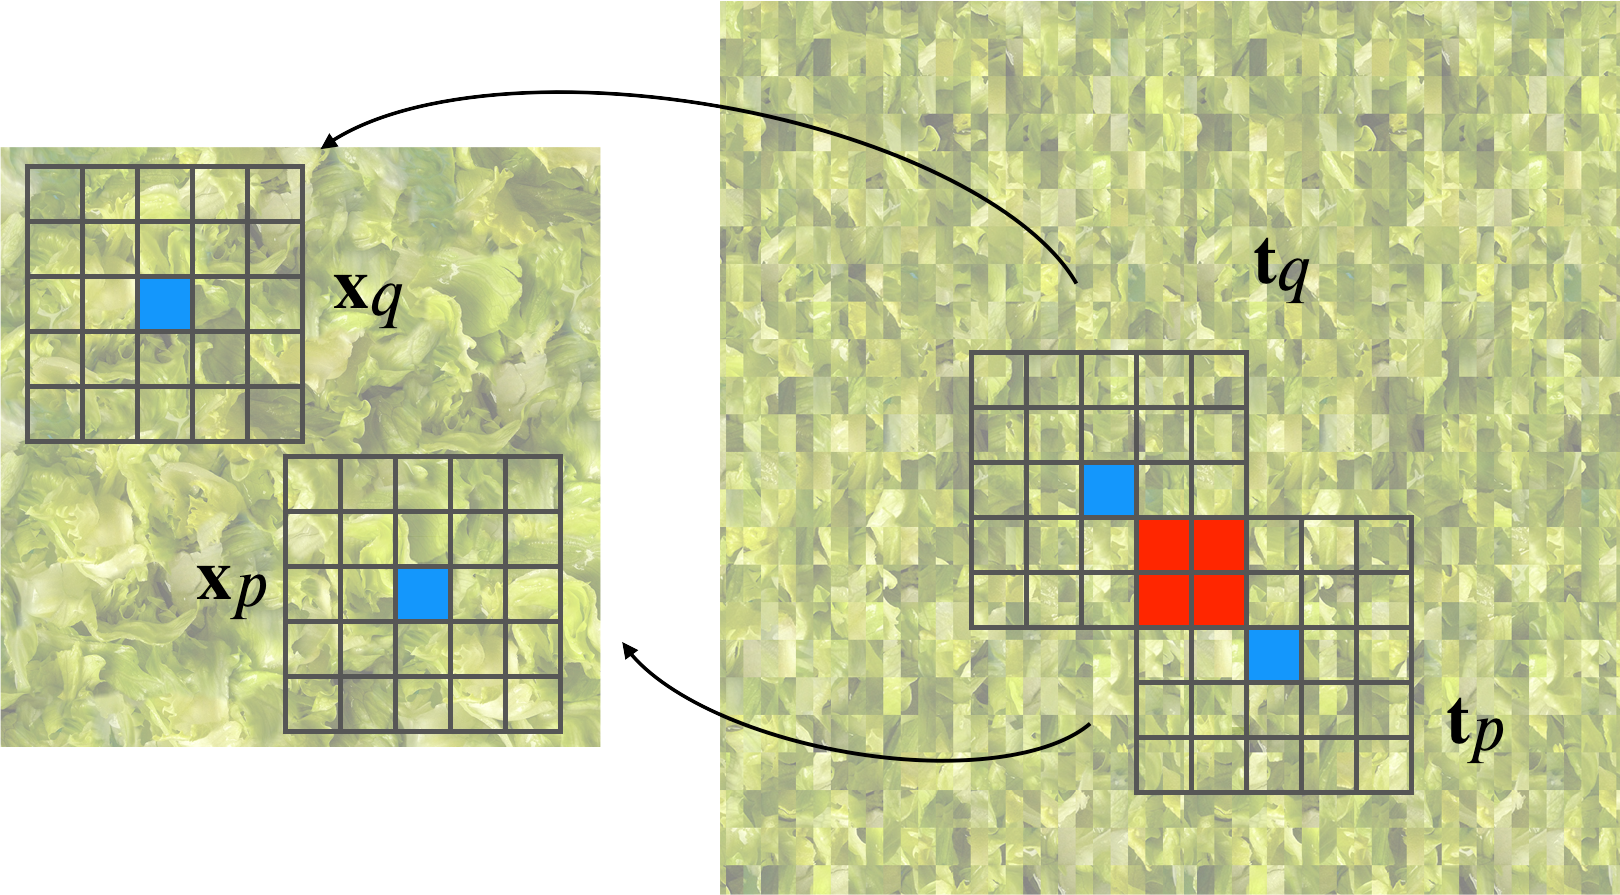
\includegraphics[width=0.7\textwidth]{images/texture-optimization}
	\caption{
		Zwei überlappende Nachbarschaften $\textbf{t}_p$, $\textbf{t}_q$ in der Textur und deren ähnlichste Nachbarschaften $\textbf{x}_p$, $\textbf{x}_q$ im Beispielmuster.
		Wenn sich zwei Nachbarschaften überlappen (roter Bereich), dann führt jede Diskrepanz zwischen $\textbf{x}_p$ und $\textbf{x}_q$ in diesem Bereich zu einem Fehler in der synthetisierten Textur.
		}
	\label{texturoptimierung}
\end{figure}

Es ist wichtig anzumerken, dass dabei nur eine Teilmenge an Pixeln $p \in T^{\dagger} \subseteq T$ aus der Textur berücksichtigt wird.
Es zeigt sich, dass die Berachtung aller Pixel in $T$ redundant ist und sich daher berechnungstechnisch nicht lohnt \cite{TextureOptimization}.
$T^{\dagger}$ wird dabei so gewählt, dass sich die Nachbarschaften benachbarter Pixel überlappen.
Damit beeinflussen nur eine Handvoll an Nachbarschaften die Farbe eines gegebenen Pixels.
Das verhindert, dass Pixel in Regionen, die sich in vielen Nachbarschaften überlappen, im Endresultat zu verwaschen wirken \cite{TextureOptimization}.

Die Textursynthese nutzt die Zielfunktion (\ref{zielfunktion}) um $T$ sukzessive zu optimieren, in dem $E$ über mehrere Iterationen minimiert wird.
Dafür wird die Zielfunktion alternierend zwischen ihren beiden Eingabeparametern $T$ und $\lbrace \textbf{x}_p \rbrace$ minimiert.
Im ersten Schritt wird die Menge $\lbrace \textbf{x}_p \rbrace$ bestimmt, sodass für alle $\textbf{t}_p$ mit $p \in T^{\dagger}$ gilt, dass $d(\textbf{t}_p, \textbf{x}_p)$ minimal ist.
So werden die ähnlichsten Nachbarschaften im Beispielmuster zu allen betrachteten Nachbarschaften in $T$ gefunden.
Damit kann folglich $T$ aktualisiert werden, sodass $E$ mit den gefundenen $\lbrace \textbf{x}_p \rbrace$ minimal ist.
Durch die Aktualisierung von $T$ können sich wiederum die ähnlichsten Nachbarschaften $\lbrace \textbf{x}_p \rbrace$ zu dem aktualisierten $T$ verändert haben und die Minimierung beginnt mit den neuen Eingaben von vorne.
Sie wird solange wiederholt, bis sich die Menge $\lbrace \textbf{x}_p \rbrace$ nicht mehr verändert (vgl. \cite{TextureOptimization}).

Die Lösung dieses Minimierungsproblems basiert auf dem \emph{\glqq Expectation-Ma\-xi\-mi\-za\-tion (EM)\grqq} -Algorithmus (vgl. \cite{EM}).
Der EM-Algorithmus findet Anwendung, wenn zusätzlich zu dem Problem der Optimierung der Zielfunktion dessen Parameter an die neue Zuordnung angepasst werden müssen.
Das unterteilt die Lösung des Minimierungsproblems in zwei Schritte.

Der \emph{E-Schritt} minimiert die Zielfunktion, in dem ein neues $T$ bestimmt wird, sodass $d(\textbf{t}_p, \textbf{x}_p)$ minimal ist für alle $p \in T^{\dagger}$.
Für Pixel in der Textur, die lediglich einer Nachbarschaft angehören, bedeutet das insbesondere, dass diese die Farbe des Pixels an der Position im entsprechenden Beispielmuster annehmen.
Für Pixel, die sich in mehreren Nachbarschaften wiederfinden (vgl. roter Bereich in Abbildung \ref{textureopimization}), wird dessen neue Farbe über die Mittelung der verschiedenen Pixelfarben aus den zugehörigen Nachbarschaften des Beispielmusters bestimmt \cite{TextureOptimization}.
Diese Mittelung führt zu einer gewissen Unschärfe und erlaubt dem Optimierungsprozess, neue ähnliche Nachbarschaften im Beispielmuster zu finden.

Der \emph{M-Schritt} ändert schließlich die Parameter für das aktualisierte $T$, in dem für das festgehaltene $T$ dessen neue ähnlichste Nachbarschaften im Beispielmuster gesucht werden.
Dies beinhaltet die Lösung eines klassischen \emph{\glqq Nearest Neighbor Search\grqq} -Problems (vgl. \cite{TextureOptimization}).

Das beschriebene Verfahren der Texturoptimierung aus \cite{TextureOptimization} wiederholt die Synthese der Textur mit unterschiedlichen Nachbarschaftsgrößen.
Die Synthese beginnt großflächig mit einer Nachbarschaftsgröße von $32 \times 32$ Pixeln.
Das gibt der Textursynthese ein anfängliches Gefühl eines regionsbasierten Verfahrens und erlaubt damit, dass auch größere Strukturen vom Beispielmuster an die zu synthetisierende Textur übergeben werden können \cite{TextureOptimization}.
Die Textursynthese wird anschließend durch kleinere Nachbarschaftsgrößen verfeinert ($16 \times 16$, $8 \times 8$, ...).
Damit gleicht der Optimierungsprozess einer \emph{Scale-Pyramide} \cite{SelfTuning}, der nach und nach über verschiedene Skalierungen der Nachbarschaftsgrößen verfeinert wird.
Mittels dieses Verfahrens entfällt ebenso die benutzerdefinierte Eingabe einer passenden Nachbarschaftsgröße.
